% cpedoc.tex V2.0, 13 May 2010

\documentclass[times]{cpeauth}

\usepackage{moreverb}
\usepackage{xspace}

\newif\ifdraft
\drafttrue
\ifdraft
\newcommand{\onote}[1]{ {\textcolor{cyan} { (***Ole: #1) }}}
\newcommand{\terminology}[1]{ {\textcolor{red} {(Terminology used: \textbf{#1}) }}}
\newcommand{\owave}[1]{ {\cyanuwave{#1}}}
\newcommand{\jwave}[1]{ {\reduwave{#1}}}
\newcommand{\alwave}[1]{ {\blueuwave{#1}}}
\newcommand{\jhanote}[1]{ {\textcolor{red} { ***shantenu: #1 }}}
\newcommand{\alnote}[1]{ {\textcolor{green} { ***andreL: #1 }}}
\newcommand{\amnote}[1]{ {\textcolor{blue} { ***andreM: #1 }}}
\newcommand{\smnote}[1]{ {\textcolor{brown} { ***sharath: #1 }}}
\newcommand{\pmnote}[1]{ {\textcolor{blue} { ***Pradeep: #1 }}}
\newcommand{\msnote}[1]{ {\textcolor{cyan} { ***mark: #1 }}}
\newcommand{\note}[1]{ {\textcolor{magenta} { ***Note: #1 }}}
\else
\newcommand{\onote}[1]{}
\newcommand{\terminology}[1]{}
\newcommand{\owave}[1]{#1}
\newcommand{\jwave}[1]{#1}
\newcommand{\alnote}[1]{}
\newcommand{\amnote}[1]{}
\newcommand{\athotanote}[1]{}
\newcommand{\smnote}[1]{}
\newcommand{\pmnote}[1]{}
\newcommand{\jhanote}[1]{}
\newcommand{\msnote}[1]{}
\newcommand{\note}[1]{}
\fi

\newcommand{\pilot}{Pilot\xspace}
\newcommand{\pilots}{Pilots\xspace}
\newcommand{\pilotjob}{Pilot-Job\xspace}
\newcommand{\pilotjobs}{Pilot-Jobs\xspace}
\newcommand{\pilotcompute}{Pilot-Compute\xspace}
\newcommand{\pilotmapreduce}{PilotMapReduce\xspace}
\newcommand{\pilotdata}{Pilot-Data\xspace}
\newcommand{\pd}{PD\xspace}
\newcommand{\pj}{PJ\xspace}
\newcommand{\pjs}{PJs\xspace}
\newcommand{\pds}{Pilot Data Service\xspace}
\newcommand{\computeunit}{Compute-Unit\xspace}
\newcommand{\computeunits}{Compute-Units\xspace}
\newcommand{\dataunit}{Data-Unit\xspace}
\newcommand{\dataunits}{Data-Units\xspace}
\newcommand{\du}{DU\xspace}
\newcommand{\dus}{DUs\xspace}
\newcommand{\cu}{CU\xspace}
\newcommand{\cus}{CUs\xspace}
\newcommand{\su}{SU\xspace}
\newcommand{\sus}{SUs\xspace}
\newcommand{\schedulableunit}{Schedulable Unit\xspace}
\newcommand{\schedulableunits}{Schedulable Units\xspace}
\newcommand{\cc}{c\&c\xspace}
\newcommand{\CC}{C\&C\xspace}

\usepackage[
%dvips,
colorlinks,bookmarksopen,bookmarksnumbered,citecolor=red,urlcolor=red]{hyperref}

\newcommand\BibTeX{{\rmfamily B\kern-.05em \textsc{i\kern-.025em b}\kern-.08em
T\kern-.1667em\lower.7ex\hbox{E}\kern-.125emX}}

\def\volumeyear{2012}



\begin{document}

\runningheads{S. Jha et al.}{Pilot-Abstractions for MapReduce-based  Cloud Applications}

\title{Pilot-Abstractions for MapReduce-based Cloud Applications}

%on Clouds and Grids}

%Extensible, Scalable, Interoperable 

\author{Andre Luckow, Pradeep Mantha, Melissa Romanus, Shantenu
  Jha\corrauth}

\address{Radical Research Group, Rutgers University}

\corraddr{Journals Production Department, John Wiley \& Sons, Ltd,
The Atrium, Southern Gate, Chichester, West Sussex, PO19~8SQ, UK.}

\begin{abstract}

The data generated by scientific applications is experiencing an
exponential growth; there exists a risk that the ability to analyze it
successfully may lag. Efficient and integrated analytical capabilities
that support scalable and advanced analytics whilst supporting
interoperability and extensibility are required; this includes runtime
environments and methods that can exploit them.  In addition to being
effective on localized data, MapReduce can when used in conjunction
with appropriate runtime environments, be used to efficiently process
distributed data across a distributed set of resources.  Specifically,
in recent work we demonstrated precisely such capabilities, viz.,
showed how Pilot-MapReduce --- a flexible, infrastructure-independent
runtime environment for MapReduce was able to address the
data-analytic requirements for a large-scale problem for both local
and distributed data.  PMR is based on Pilot-abstractions for compute
(Pilot-Jobs) and data (Pilot-Data). Pilot-Jobs are used to couple the
map phase computation to the nearby source data, and Pilot-Data is
used to move intermediate data using parallel data transfers to the
reduce computation phase.  This work builds upon earlier work to show
how Pilot abstractions and PMR enable the processing of distributed
data across multiple heterogeneous distributed infrastructure,
including concurrent usage of clouds and traditional
grids/clusters. We further show how PMR can efficiently support
different infrastructure and application characteristics, We further
analyze different resource topologies and MapReduce configuration,
such as both hierarchical and iterative MapReduce. In particular, we
investigate typical infrastructure trade-offs (e.g. the overhead times
in spawning virtual machines, the geographic distribution, etc).

\end{abstract}

\keywords{MapReduce; Grid Computing; Cloud Computing; Data-Intensive; Compute-Intensive}

\maketitle

\footnotetext[2]{Please ensure that you use the most up to date
class file,
available from the CPE Home Page at\\
\href{http://www3.interscience.wiley.com/journal/117946197/grouphome/home.html}{\texttt{http://www3.interscience.wiley.com/journal/117946197/grouphome/home.html}}}

\vspace{-6pt}

\section{Introduction}
\vspace{-2pt}

\jhanote{In general: no references in abstract: \pilotmapreduce
  (PMR)~\cite{Mantha:2012:PEF:2287016.2287020} } \jhanote{last few
  sentences of abstract need fixing}


\begin{verbatim}

Application perspective versus Infrastructure perspective: (I)
 Application Motivation/Challenges: Scaling data intensive
 applications - Why is this a problem? Any real application requires
 this problem to be solved?  - CMS, Atlas generates PBs of data/ day.
  (II) Infrastructure Motivation: Emerging infrastructure, data
 oriented infrastructure, scalability of infrastructure, possibly
 better abstractions and capabilities.

Note our focus and context: (i) distributed data scenarios (ii) pilot
 abstraction to address heterogeneity, scalability and extensibilty

Some Research Questions: (i) How does Pilot-Abstraction work in the
 clouds (we've addressed pilot-jobs before, now focus on pilot-data)
 (ii) how to address data distribution in the cloud? (iii) cloud data
 localization requirements: how and when does that become a barrier?
  (iv) related to previous, Can we say something when to use cloud or
 When Grid?

\end{verbatim}

\jhanote{Other Issues worth mentioning: not sure what these are tying
 to say: Does minimizing queue wait time, distributed nature of
 Pilot-abstractions motivate Domain Scientists to use freely available
 Grid resources?  Waiting time and cost increases as Number of
 instances required increase?  HOw is it beneficial than Grids?}


\pmnote{ Scientists believe clouds provide computing infrastructure on demand with minimal or negligible waiting time..  Production cyberinfrastructures involve waiting time if they don't take advantage of Pilot abstractions...  So, what I want to say is- scientists are ignoring existing abstractions and simply moving to cloud.. Is that because of hype? }

\note{Why Domain scientists are moving to cloud? Hype? Due to
  non-availability of necessary simple abstractions to scale
  applications on Grid?} \jhanote{I don't think we should be making
    that argument here for it undermines our own point of view that
    Pilot abstractions have been relatively / modestly successful on
    grids}

\pmnote{ I mean , Given the success the Pilot abstractions on Grids , Domain scientists should start using Pilot abstractions rather than using on demand cloud services - which are expensive - I think its an opportunity to exploit the importance of BigJob and SAGA;  Can we mention some usecases where PJ's effectively supported real science(Tom Bishop usecase)? 
I think as PJ's popularity increases - requirement to use clouds decreases ( since no waiting time between compute units) )}
\pmnote{Does clouds support real science}

\note{These are design objectives: Interoperability, Scalability,
  Extensibility/Flexibility/usability}

%\note{Not in scope any more: Why Iterative MapReduce?What
%  Application?  ( k-means?)Why k-means?  - twister mapreduce used
%  k-means?  - k-means implemented using windows azure}

% Definition
A Pilot-Job provides the ability to utilize a placeholder job as a container 
for a dynamically determined set of compute tasks.

\section{The Case for Distributed, Data-intensive Computing}

What are our contributions, challenges of distributed, data-intensive computing?
\begin{itemize}
	\item choosing the right cloud... 
	\item how to couple different clouds
	\item transport in and out to cloud
	\item support late-binding: late binding as a fundamental attribute in 
	distributed systems
\end{itemize}
Pilot-Jobs help us to address these requirements.

\section{Related Work}

Prior Work (Pradeep)

Distributed CyberInfrastructure is dynamic and also involve widely distributed heterogenous computing and storage clusters. Pilot abstractions proved to be effective on DCI for distributed compute and data management. On the other hand, MapReduce programming model is a popular solution for distributed data processing and involves map and reduce (compute) phases, and a shuffle (data movement) phase. Traditional MapReduce implementations like Hadoop are typically designed for single clusters and when scaled across widely distributed clusters lead to performance problems. Deployment of Hadoop cluster on shared dynamic resource pool also involves manual management of compute and data resources and managing workflows  involving MapReduce execution patterns becomes tedious. Policies of cyberInfrastructures doesn't allow to execute Hadoop on more than one cluster. These limitations of traditional implementations motivated to develop a Pilot abstractions based MapReduce programming model - Pilot-MapReduce for distributed data analysis.

Pilot-MapReduce decouples the logic/pattern of MapReduce from
the actual management of the distributed compute, data and network resources. By
decoupling job scheduling and monitoring from the resource management,
PMR can efficiently reuse the resource management and late-binding
capabilities of BigJob and BigData, which are SAGA based Pilot-Job and Pilot-Data implementations.

PMR exposes an easy-to-use interface which provides the complete
functionality needed by any MapReduce-based application, while hiding
the more complex functionality, such as chunking of the input, sorting
the intermediate results, managing and coordinating the map and reduce
tasks, etc., these are generically implemented by the
framework~\cite{pmr2012}.



Related Work (Melissa)

\begin{itemize}
	\item Coaster
	\item Venus C (Generalized Worker)
\end{itemize}


\section{Cloud Computing and Cloud-based Infrastructures}

At a high level, cloud computing is defined by Mell/Grance~\cite{nist_cloud}
as a model for enabling convenient, on-demand network access to a shared pool
of configurable computing resources (e.g., networks, servers, storage,
applications, and services) that can be rapidly provisioned and released with
minimal management effort or service provider interaction.

\alnote{Do we want to talk about the ``old'' SaaS, PaaS and IaaS stuff?}

Talk about the evolution of PaaS and IaaS towards general services/building 
blocks

Amazon API
GData API
OpenStack API
OCCI


Commercial Clouds vs. Science Clouds


Frameworks such as OpenStack~\cite{openstack} and Eucalyptus~\cite{euca} aim
to provide a framework for building a private cloud environment which similar
capabilities as EC2 and S3. FutureGrid's cloud environment currently supports
both framework.

\begin{itemize}
	\item Resource Model
	\item Provisioning Model
	\item Business Model
\end{itemize}

\subsection{Cloud Storage Services}

An important component for data-intensive cloud applications are the cloud
storage services. Many clouds offers various kinds of storage services with
different characteristics, e.\,g.\ these services usually differ in their read
and/or write performance, supported data volumes, interfaces, reliability and
scalability (see Baron~\cite{baron2010} for an overview of Amazon's storage
services). While clouds often provide storage services on different 
abstraction levels (including e.\,g.\ relation databases), in the following we 
focus on general file-based storage types. In general, cloud storage can be 
classified as follows:
\begin{enumerate}
	\item \textbf{Local Storage:} describes local hard disk directly attached 
	to the compute resource.
	\item \textbf{Network-attached Filesystems:} refers to different forms of 
	distributed (possible parallel) filesystems. The filesystem is commonly 
	exported via the Posix API and a virtual filesystem layer.
	\item \textbf{Distributed Storage:} refers to a highly distributed type of 
	storage systems that spawn across multiple data centers. Access to such 
	storage systems via a common -- often simplified -- namespace and API. For 
	example, cloud systems, such as the Azure Blob Storage, Amazon S3 and 
	Google Storage, provide only a namespace with a 1-level hierarchy. 
\end{enumerate}

A particular novelty for clouds are distributed storage services, such as
Amazon S3, Google Storage and the Azure Blob storage. The storage systems are
optimized for storing large volumes of data and for achieving high
read throughputs. For example, Amazon S3 automatically replicates data across 
multiple data centers within a region. 


Table~\ref{tab:storage-systems} shows an overview of distributed storage 
systems. The focus of this analysis are file-based storage systems. Structured
storage types (e.g. relational databases) and key-/values stores are not 
considered.

\begin{table}[t]
\centering
\begin{tabular}{|p{1.7cm}|p{1.3cm}|p{1.3cm}|p{1.3cm}|p{1.4cm}|p{1.4cm}|p{1.3cm}|p{1.2cm}|}
	\hline
	\textbf{Storage Type} &\textbf{Azure} &\textbf{Amazon} &\textbf{Google} &\textbf{Open\-Stack} &\textbf{Euca\-lyptus} &\textbf{XSEDE}  &\textbf{OSG} \\
	\hline
	Local	&yes &yes &yes &yes &yes &yes &yes\\
	\hline
	Network Filesystem &Azure Drive &EBS &GCE Block Storage &Nova Volumes &? &Lustre, GPFS 
	&no\\
	\hline
	Distributed Storage &Azure Blob Storage &S3 &Google Storage &Swift & Walrus &GFFS
	 &SRM\\
	\hline	
\end{tabular}
\caption{File-based storage types for different infrastructures (key/value and 
SQL-based storage types omitted) \label{tab:storage-systems}}
\end{table}


% Limitations
While some cloud services that support a high degree of geographic 
distribution have emerged, e.\,g.\ content delivery services such as Akamai 
and Amazon CloudFront, dealing with geographically distributed data remains a 
challenge. However, both Google and Facebook internally deploy systems that 
supports the management of large data volumes across multiple, geographically
dispersed locations. Both Google Spanner~\cite{dean09} and Facebook 
Prism~\cite{Metz12} aim to provide one logical namespace and handle the 
automatic replication and movement of data. However, these capabilities are 
currently not available as external cloud services. If an application requires 
such capabilities, it needs to implement these manually. In this paper we show 
how \pilot abstractions can help to manage geographically distributed data.


\subsection{Data-intensive Applications}

Scenarios
\begin{itemize}
	\item Data is in the cloud or can be brought to the cloud
	\item Distributed data: data resides on different infrastructures, different resources (within a cloud)
\end{itemize}


\subsubsection{Hadoop in the Cloud}

\alnote{How do the different cloud providers chose to re-package Hadoop and 
provide an integrated service?}

\begin{itemize}
	\item Elastic MapReduce
	\item Hadoop on Azure
\end{itemize}

\subsubsection{Other Applications}

1000 Genome project





\section{Pilot Abstractions for Clouds}

% Intro to P* model
The P* model~\cite{pstar12} is an attempt to provide the first minimal but
complete model for describing and analyzing \pilotjobs. The P* model defines
common elements of both compute and data pilot implementations. In this 
section we show how the unified pilot abstractions can be used to support 
data-intensive applications in clouds as well as hybrid grid/cloud 
environments.


\subsection{Motivation}

% Why pilot abstractions for clouds?
\begin{itemize}
	\item Cloud/Grid interoperability
	\item Hybrid infrastructures 
	\item Pilots as resource management abstraction (scheduling, affinities)
	\item Pilots as basis for building capabilities in grids/clouds (PMR as 
	example)
\end{itemize}


Pilot-Jobs decouple resource allocation from resource binding and allow the 
efficient utilization of resources. Pilot-Jobs are an execution abstraction 
that has been used by many communities to (i) improve the utilization of 
resources, (ii) to reduce wait times of a collection of tasks, (iii) to 
facilitate bulk or high-throughput simulations where multiple jobs need to be 
submitted which would otherwise saturate the queuing system, and (iv) as a 
basis to implement application specific scheduling decisions and policy 
decisions.


Pilot abstractions provide a suitable mean to marshall heterogeneous sets of 
both compute and data resources and support the efficient utilization of 
different kinds of commercial as well science cloud resources.


Describe job and data perspective for each of these points
submit to clouds through grids (e.g. OSG/EGI)
Cloud bursting as use case
Data perspective to hybrid infrastructure: data-distribution problem requires different kinds of operations

distributed cyberinfrastructures via the use of an extensible API for the P* Model (Pilot-API).
timeframe of infrastructure change is much larger than for application change
Does the api evolvement make it difficult to applications to follow: what 
about apps that want to use EUCA, OpenStack


\subsection*{Data Management in the Cloud}

In general, the following strategies for managing compute and
data in distributed environments exist:

\begin{itemize}
\item A: Data is naturally distributed, processing happens locally to the data. 
\item B: Data is originally localized, but the data needs to be distributed to match the distribution of compute resources.
\item C: Data is moved so as to be localized (i.e., raw data is moved)
\end{itemize}

In most cases, application data is initially pushed to a cloud storage 
service, such Amazon S3, Google Storage and Azure Storage. These service, such 
as S3, are well suited for storing large amounts and support typical 
data-intensive workloads (e.\,g.\ with a lot of sequential reads)

Recently, various markets for data in the cloud have emerged. Cloud providers,
such as Amazon and Microsoft published various scientific data set in these
markets. Amazon e.\,g.\ provides access to various datasets of the 1000 genome
project.


We want to use hybrid infrastructures in all of these modes 



\subsection{BigJob and BigData for Clouds}

Pilot-Data provides a unifying interface to a heterogeneous set of data 
sources removing the need to interoperate with different data sources, e.\,g.\ 
repositories, databases etc, providing a virtualized data service layer.

\begin{figure}[t]
	\centering
		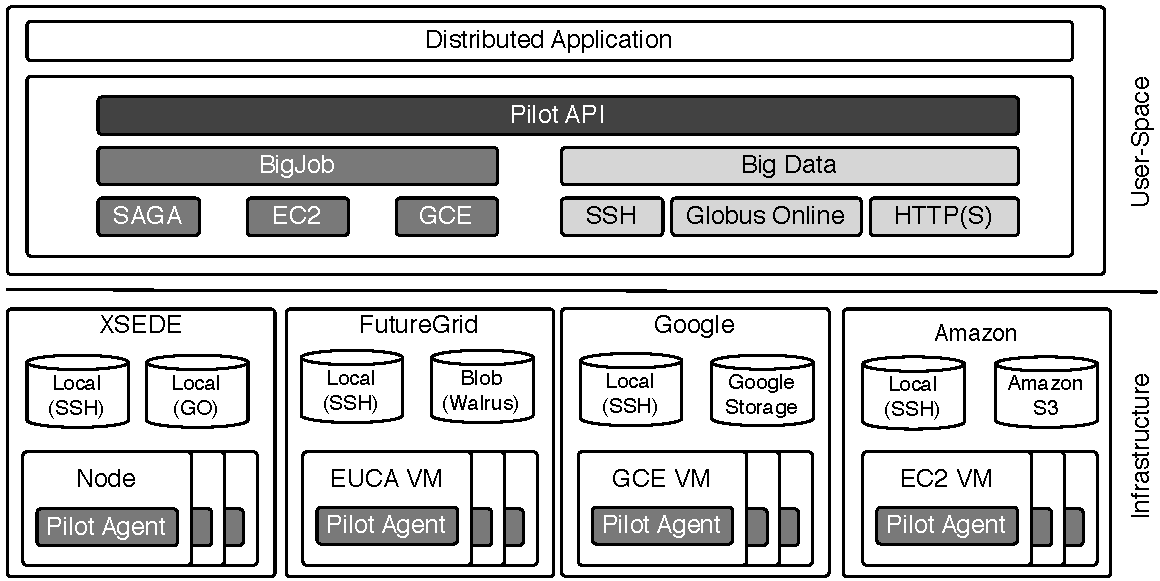
\includegraphics[width=0.7\textwidth]{figures/cloud_pilot_job.pdf}
	\caption{Pilot Abstractions and Clouds\alnote{todo: differentiate between 
	storage and transfer protocol}}
	\label{fig:figures_cloud_pilot_job}
\end{figure}

Figure~\ref{fig:figures_cloud_pilot_job} shows how the Pilot-API and 
BigJob/BigData can be used to manage a heterogenous set of both cloud and grid 
resources. BigJob supports various resource types via a flexible plugin 
architecture. In addition to SAGA, BJ can natively utilize both the EC2 and 
GCE API to launch BJ agents. Similarly, BigData supports various data access
protocols and storage types -- currently, SSH, Globus Online, Google Storage
and Amazon S3.



\begin{figure}[t]
	\centering
		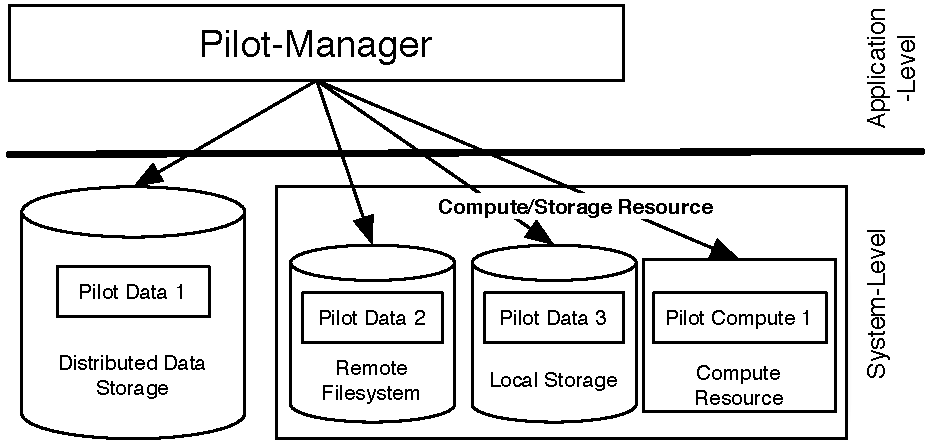
\includegraphics[width=0.7\textwidth]{figures/storage-types.pdf}
	\caption{Pilot-Compute and Pilot-Data on Different Types of Storage Resources}
	\label{fig:figures_storage-types}
\end{figure}

The aim of Pilot abstractions is to marshal the differences in the different 
cloud storage types (see Figure~\ref{fig:figures_storage-types}) and aims to 
provide a unified interface to these services. Affinities are an essential 
tool for modeling the different storage characteristics and to allow an 
effective reasoning about different storage topologies and data/compute 
placements.


Figure~\ref{fig:figures_data-flow} shows the interactions and the data flow 
between \computeunits and \dataunits.
\begin{figure}[htbp]
	\centering
		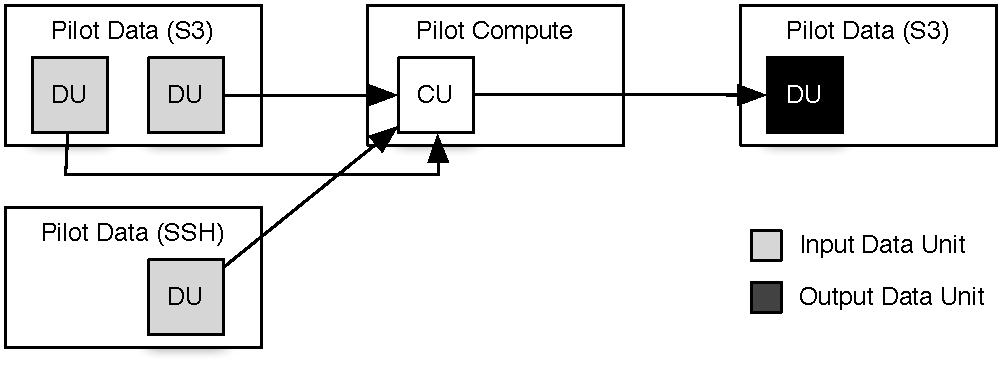
\includegraphics[width=0.7\textwidth]{figures/data-flow.pdf}
	\caption{DU and CU Interactions and Data Flow}
	\label{fig:figures_data-flow}
\end{figure}



\section{Pilot-MapReduce for Clouds}

Pilot-MapReduce is a pilot-based implementation of the MapReduce
programming model, which decouples the logic/pattern of MapReduce from
the actual management of the compute, data and network resources. By
decoupling job scheduling and monitoring from the resource management,
PMR can efficiently reuse the resource management and late-binding
capabilities of BigJob and BigData.

PMR exposes an easy-to-use interface which provides the complete
functionality needed by any MapReduce-based application, while hiding
the more complex functionality, such as chunking of the input, sorting
the intermediate results, managing and coordinating the map and reduce
tasks, etc., these are generically implemented by the
framework~\cite{pmr2012}.


\alnote{Add layered diagram (incl. PMR) of software stack for different 
infrastructures}
\pmnote{ is it just adding a Pilot-MapReduce layer to Fig:1 ? }

\section{Experiments}

\subsection{Infrastructure}

Compute:
\begin{itemize}
	\item FutureGrid/XSEDE: Sierra, Kraken 
	\item FutureGrid India/Eucalyptus
	\item FutureGrid India/OpenStack
\end{itemize}

Data:

	
\subsection{Word Count}

Experiments:
\begin{itemize}
	\item  Scale input data: 1GB, 10GB, 100GB, 1000 GB
	\item  Different amounts of intermediate data: 1GB, 10GB, 100GB, 1000 GB
	\item  Number of Resources: 1, 2, 4, 8, 16, 32 VMs
\end{itemize}

\subsection{NGS}

\section{Conclusion and Future Work}

\bibliographystyle{wileyj}
\bibliography{literatur,saga,saga-related,local}

\end{document}
